%!TEX root = ../main.tex

\section{Voronoi diagram generation and Lloyd relaxation}
\label{sec:lloyd_relaxation}

In order to position more evenly the sites, we apply a Lloyd relaxation scheme based on 3D geodesic distances, using the connectivity of the depthmap.
This algorithm is decomposed into two steps : 

\begin{itemize}
	\item Computing a voronoi diagram, determining for each site $s_i$ the closest points from $s_i$ to any other site.
	\item Integrating each cell of the Voronoi diagram and computing its centroid.
	\item Moving the position of each site $s$ with respect to the centroid computed for its cell.
\end{itemize}

Those steps are repeated until the sites stop moving (in practice, the process is stopped when the mean displacement is below a given threshold).

\subsection{Voronoi diagram generation}
Voronoi diagrams \cite{Vor08} are a partition of a space $\mathbb{R}^n$ in a set of convex cells $V_S(v_i)$ from $k$ sites where every element contained in the cell $V_S(v_i)$ is closer from the site $v_i$ than from any other site $v_j$

\begin{equation}
\label{eq:voronoi_cell}
	V_S(v_i) = \{ x \in \mathbb{R}^n, \forall p \in S\, d(v_i,p) \leq d(v_j,p), j \neq i\},
\end{equation}

where $d$ is a distance metric. Generally, the euclidean distance metric is used to partition the domain, however it is possible to use other distance metrics (Manhattan distance, geodesic distance, ...), that will generate other partitions, depending on the needs.

To compute a Voronoi diagram over a depthmap, we use a discrete approach, through the multi-sources Dijkstra's algorithm (MSSP) \cite{Dij59} which finds for a vertex of a graph, the shortest path through the graph between this vertex and any other vertex in the graph.
We adapted a GPU implementation from the work of \cite{PPA16} to include the use of depthmaps.

This method works as a recursive process. 
At the beginning, every site $v_i$ marks the pixel it is lying on and the pixels in the 1-ring neighborhood of that pixel as being part of the Voronoi cell $V_S(v_i)$ of the site $v_i$ if their distance to that pixel is closer than any other site $v_j, j \neq i$ and marked as "ready" to propagate.
Throughout the algorithm every pixel will store its accumulated distance from the site of the Voronoi cell it belongs to. 
At the initialization this distance is set to infinity for every valid pixel of the depthmap, and set to 0 for every non-valid pixel.

Every pixel marked $p$ will check its 1-ring neighborhood and for every neighbor $p_i$, if the currently stored distance for $p_i$ $d(p_i)$ is superior to the distance stored at $p$ plus the 3D euclidian distance between $p$ and $p_i$. 
If it is the case, $p_i$ will be considered as belonging to the same cell as $p$, its stored distance being updated accordingly and it is marked as "ready" to propagate its ownership.

The algorithm stops when no pixel is marked as needing visitation anymore.

\arnaud{ADD FIGURE COMPARISON DISTANCE METRICS VORONOI (GEODESIC, EUCLIDEAN 2D)}

\subsection{Lloyd relaxation}
Now that each valid pixel of the depthmap is included in a Voronoi cell, sites are going to be moved, in order for them to be more evenly spaced locally.

Each Voronoi cell can be in two different configurations : 
\begin{itemize}
	\item \textbf{the cell doesn't touch a border}. This means that no pixel being part of the Voronoi cell belongs to the border.
	In this configuration, the cell's site is moved to the centroid of its cell
	\item \textbf{the cell touches a border}. This means that at least one pixel being part of the Voronoi cell belongs to the border.
	In this configuration, the cell's site is moved to the orthogonal projection of the centroid of the cell on the border that the cell is touching.
\end{itemize}

The new position of the  $z_i^*$ of the Voronoi cell $V_i$ can be obtained using the following integral :

\begin{equation}
		z_i^* = \begin{cases}
		Proj_{B_{V_i}}(\frac{\int_{V_S(v_i)} x\rho(x)\,dx}{\int_{V_S(v_i)} \rho(x)\,dx}) , & \text{if $|B_{V_i}| > 0$}, \\
		\frac{\int_{V_S(v_i)} x\rho(x)\,dx}{\int_{V_S(v_i)} \rho(x)\,dx}, & \text{otherwise}, 
		\end{cases}
\end{equation}

where $z^*$ is the centroid of the Voronoi cell $V_S(v_i)$ and $\rho(x)$ a probability density function defined over the domain $S$.
In our discrete case (where the domain is a depthmap), the integral can be re-written as the sum over all the pixels $p$ belonging to a Voronoi cell : 

\begin{equation}
		z_i^* = \begin{cases}
		Proj_{B_{V_i}}(\frac{\sum_{p_j \in V_S(v_i)} p_j\rho(p_j)}{\sum_{p_j \in V_S(v_i)} \rho(p_j)}) , & \text{if $|B_{V_i}| > 0$}, \\
		\frac{\sum_{p_j \in V_S(v_i)} p_j\rho(p_j)}{\sum_{p_j \in V_S(v_i)} \rho(p_j)}, & \text{otherwise}, 
		\end{cases}
\end{equation} 

We differentiate those two cases to better preserve the geometry, otherwise all the details around borders would be lost (Figure \ref{fig:borders_lloydrelaxation}).

\begin{figure}[ht]
\centering
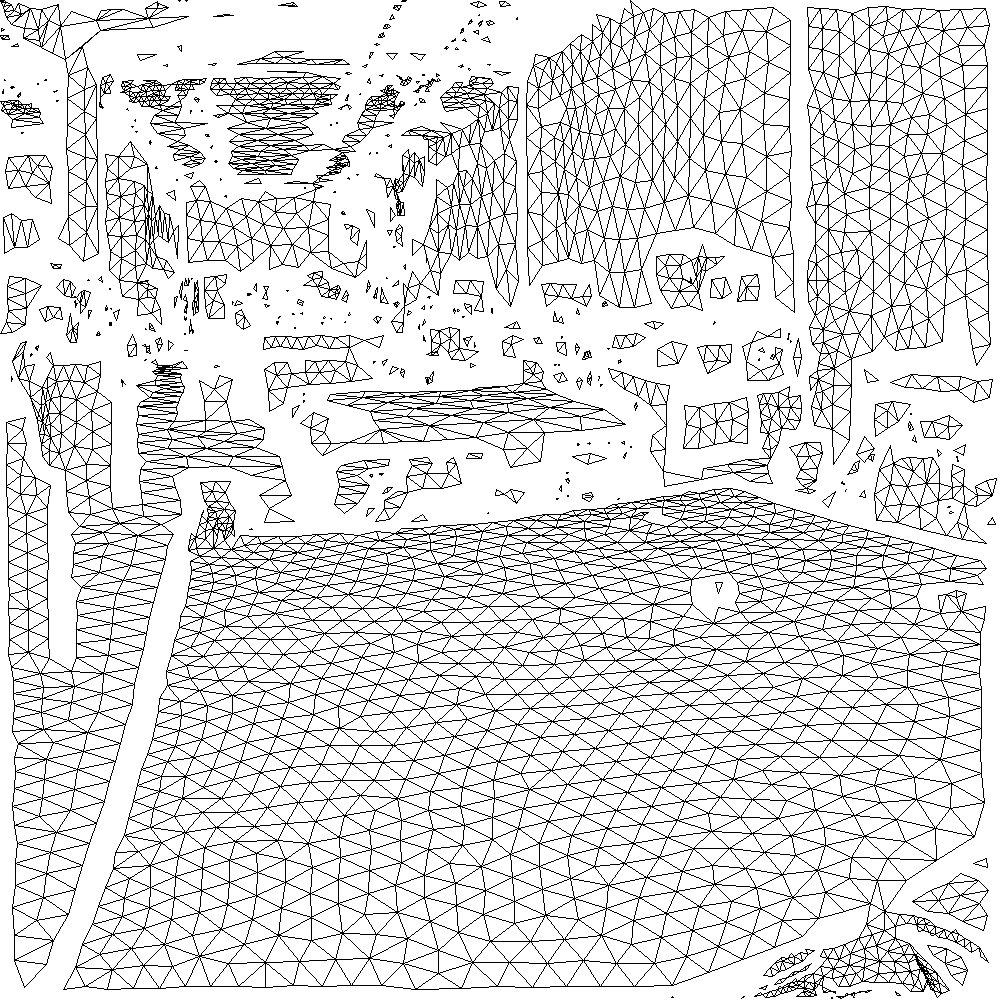
\includegraphics[scale=0.165]{Triangulation2D-LloydRelaxation-WithoutBorders-TechShop}
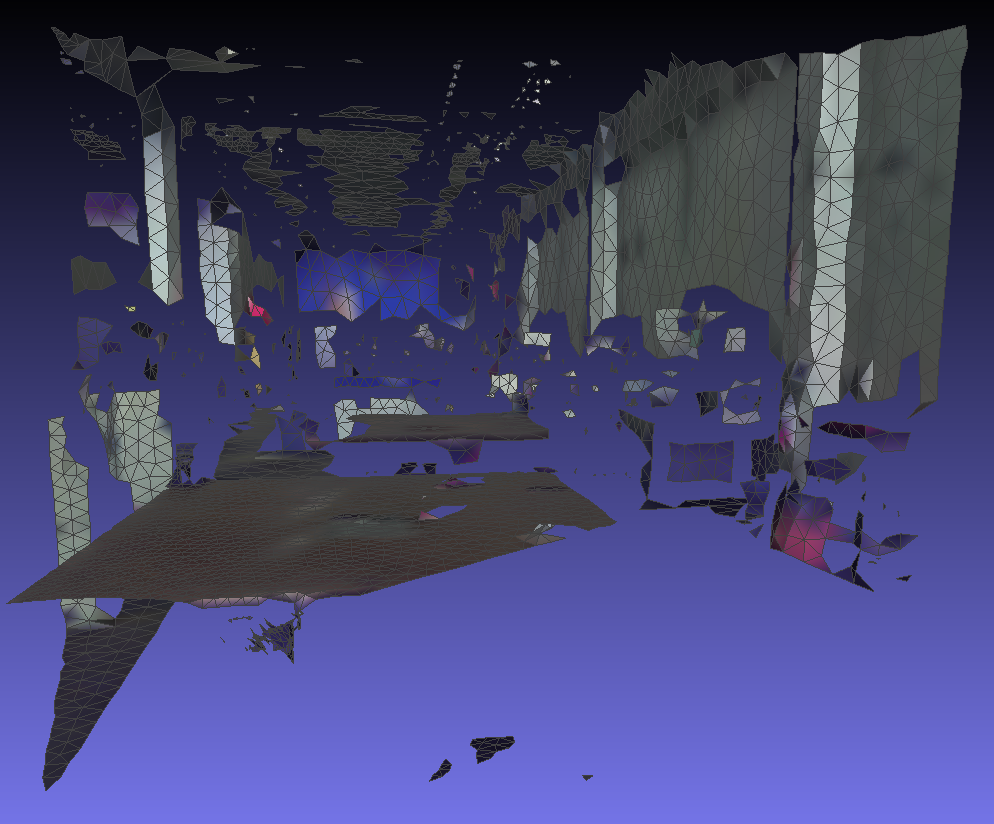
\includegraphics[scale=0.2]{Triangulation3D-LloydRelaxation-WithoutBorders-TechShop}
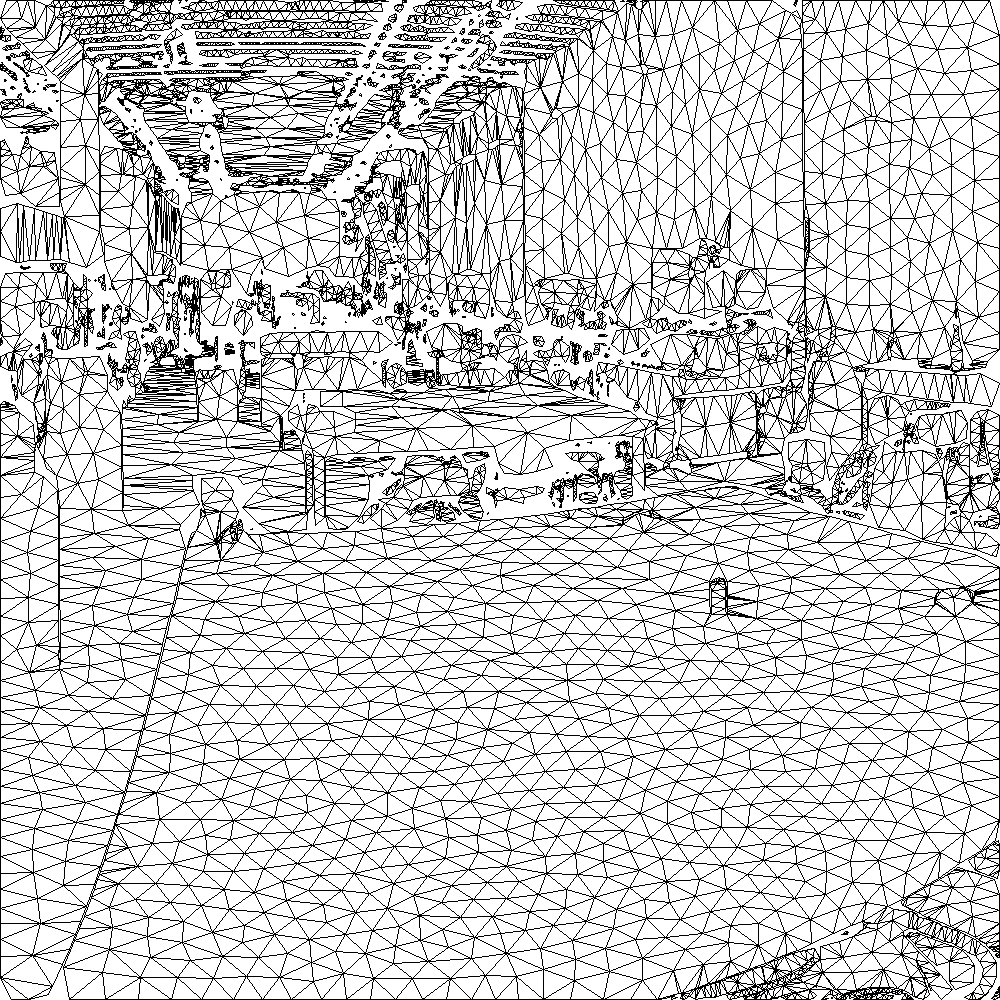
\includegraphics[scale=0.165]{Triangulation2D-LloydRelaxation-WithBorders-TechShop}
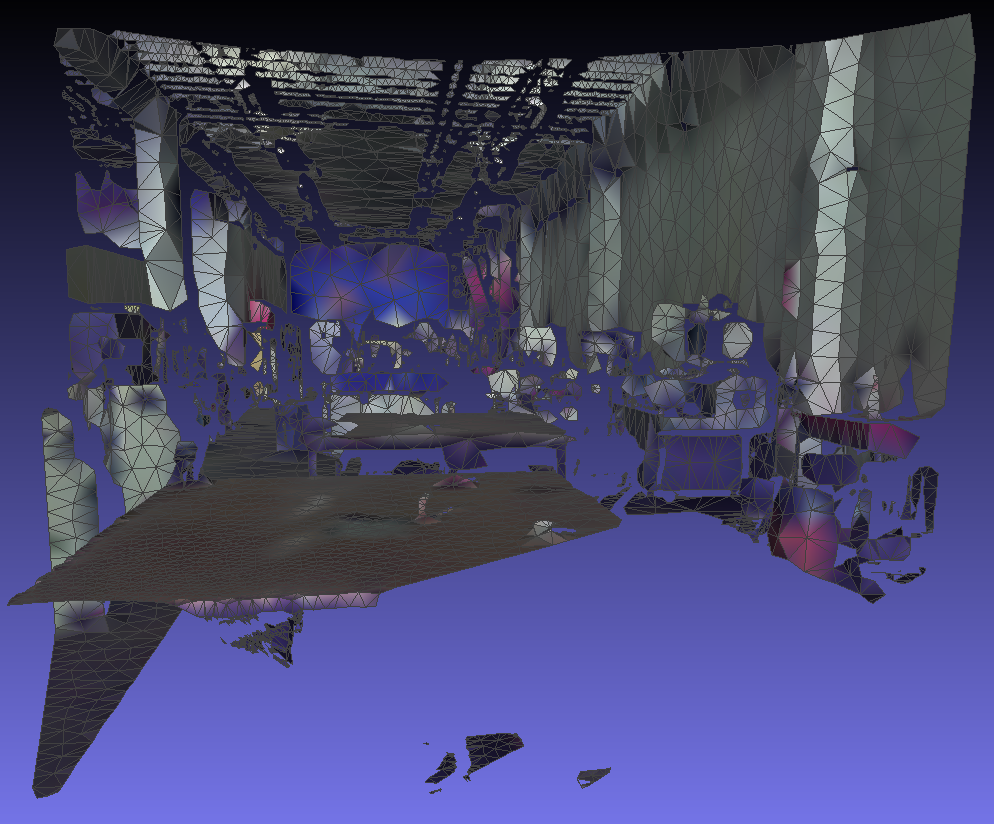
\includegraphics[scale=0.2]{Triangulation3D-LloydRelaxation-WithBorders-TechShop}
\caption{Different triangulations (in 2D on the left, in 3D on the right) obtained from a Voronoi diagram without (top part) and with (bottom part) considering the presence of borders when repositioning sites during a Lloyd relaxation procedure. When comparing the symmetric point-to-point distance between the original point cloud and the samplings obtained after the relaxation procedure (with and without borders), we obtain a RMS error respectively of $0,003404$ and $0,000677$ without and with the consideration of the borders.}
\label{fig:borders_lloydrelaxation}
\end{figure}

\subsection{Voronoi diagram verifications}
In \cite{Gus07}, verifications have been added in order to ensure that a Voronoi partition was generating a manifold mesh.
This work suggested to verify 5 different topological conditions over the configurations of Voronoi tiles (Figure \ref{fig:voronoi_conditions}) : 
\begin{itemize}
	\item \textit{Encrouched boundaries}. A Voronoi tile that touches a surface boundary has to have its seed on that boundary. 
	If this condition fails a new seed is introduced on the boundary of the surface within the current tile
	\item \textit{Nonzero genus}. A Voronoi tile needs to have zero genus. If this condition fails, a new seed is introduced at a vertex adjacent to the seed vertex of the tile.
	\item \textit{Multiple tile boundary components}. The boundary of a Voronoi tile can only consist of a single connected component. If this condition fails a new seed is introduced at a vertex adjacent to the seed vertex of the tile.
	\item \textit{Single curve tile boundaries}. A Voronoi tile that is adjacent to other tiles should not have more than one neighbor along each tile boundary curve. If this condition fails a new seed is introduced at a vertex adjacent to the tile boundary curve.
	\item \textit{Multiple neighbor instances}. Any pair of Voronoi tiles cannot touch along more than a single tile boundary curve. If this condition fails, a new seed is introduced at a vertex adjacent to the shorter among the offending tile boundary curves.
\end{itemize}

\begin{figure}[ht]
\centering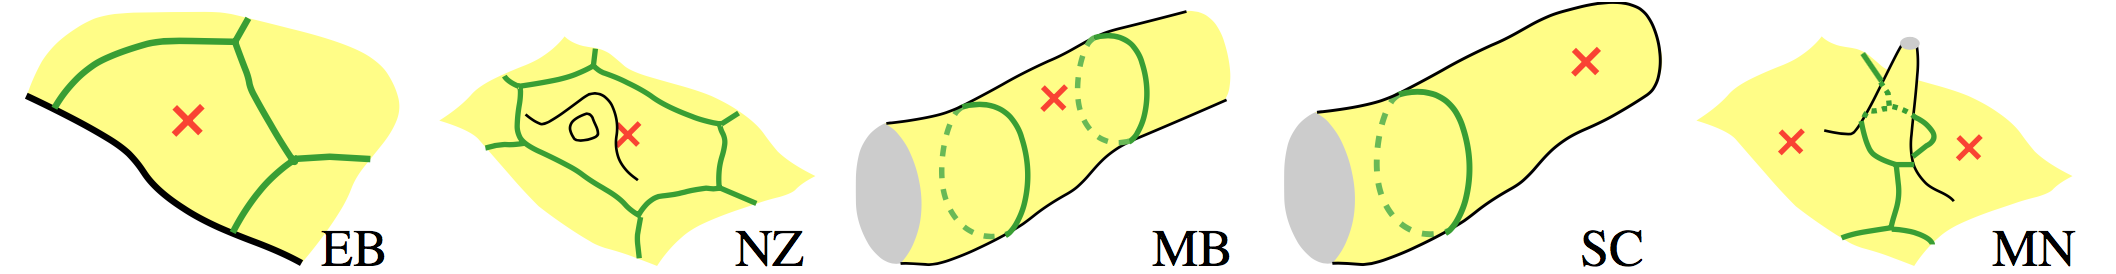
\includegraphics[scale=0.4]{VoronoiConditions}
\caption{Conditions that the Voronoi diagram has to respect in order to generate a 2-manifold triangulation (Figure from \cite{Gus07})}
\label{fig:voronoi_conditions}
\end{figure}

In our case, some configurations cannot happen.
\textit{Nonzero genus} is not a possible case, because by definition the depthmap represents the parameterization of the visible part of the scene. Thus the surface (or the multiple surface components) obtained after scanning have a zero genus and each Voronoi cell also, since each cell is a subset of the surface acquired.

Those conditions are verified after each Voronoi diagram computation.

% \subsubsection{Power diagram from Gaussian curvature}
% Power diagrams are an extension of Voronoi diagrams to represent the fact that some sites can have a higher importance than others, for them to cover a larger area with respect to their neighbors. Similarly to what has been done for the poisson sampling in Sec.\ref{sec:poisson_sampling}, where the probability density function has been weighted by the absolute Gaussian curvature of the surface, it is possible to weight the influence of the Voronoi sites by the absolute Gaussian curvature, in order to create smaller cells (smaller weight) around the surface areas which have a high absolute curvature.

% \begin{equation}
% \label{eq:power_cell}
% 	V_S(v_i) = \{ x \in \mathbb{R}^n, \forall p \in S\, d(v_i,p) - w_i \leq d(v_j,p) - w_j\}
% \end{equation}

% \arnaud{Subsubsection incomplete : more explanation about the way to compute the weights (using the curvature values) in order for the Voronoi cells size to vary smoothly.}